\chapter{Coherent Elastic Neutrino-Nucleus Scattering}
This chapter introduces the main interaction by which the sensitivities of neutrino detectors to the SM parameters are determined, describing a neutral current interaction along with its cross section, and showing how, in conjunction with a model of the antineutrino flux from a reactor source, the expected number of events for a broadly-described experimental design can be calculated; this number will be used in later chapters to test how different values of the SM parameters influence it.
\section{Introduction}
\begin{wrapfigure}{r}{0.25\textwidth}
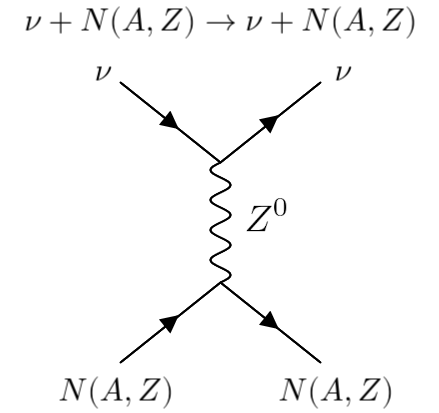
\includegraphics[width=\linewidth]{figures/feynman.png}
\label{fig:Feynmann_CEvNS}
\end{wrapfigure}
Coherent Elastic Neutrino-Nucleus Scattering (CE$\nu$NS) is a neutral current weak interaction within the SM originally proposed in 1979 \cite{PhysRevD.9.1389} and measured successfully in 2017 \cite{doi:10.1126/science.aao0990}, wherein low-energy neutrinos [$E_{\nu} \sim \, \text{MeV}$] collide with atomic nuclei as coherent bodies rather than their constituents, imparting on them a small recoil energy. These interactions are possible with neutrino energies up to $50\,MeV$ with medium-sized nuclei, since their main condition consists of the momentum transfer, $Q$, being negligible in comparison with the nuclear radius, $R$ ($QR \ll 1$) \cite{Scholberg_2020}. The effective Feynman diagram for these interactions is shown in Fig. \ref{fig:Feynmann_CEvNS}.

The calculation of its differential cross-section in the low-energy limit consists of setting an effective Lagrangian density given by:
\begin{equation}
    \mathcal{L_{\text{eff}}} = \frac{G}{\sqrt{2}}j^{(\nu)\mu} \mathcal{J}_{\mu},
\end{equation}
where $j^{(\nu)\mu}$ denotes a neutral neutrino current and $\mathcal{J}_{\mu}$ a hadronic current from which the nuclear mass distribution terms originate.
\section{Cross Section}
The low-energy differential cross-section in terms of the nuclear recoil, $E_R$, is given by \cite{Papoulias2015}:
\begin{equation}
    \frac{d\sigma}{dT}(E_\nu, E_R) = \frac{G_{F}^{2} M}{\pi}Q_{W}^{2}\left(1 - \frac{ME_R}{2E_\nu}\right),
\end{equation}
where $M$ is the target nuclear mass and $Q_W^2$ is the vector nuclear weak charge given in terms of the proton ($p$) and neutron ($n$) weak couplings:
\begin{equation}
    Q_{W}^{2} = [Zg^{p}_{V}F_p(q^2) + Ng^{n}_{V}F_n(q^2)]^2,
    \label{eq:QW}
\end{equation}
where $g^{p}_{V}$ and $g^{n}_{V}$ are given by (\ref{eq:gv}) in the specific cases for the proton and neutron respectively:
\begin{align}
    g^{p}_{V}   &= T^3_{p}-2\sin^2(\theta_W)Q_{p}   =\frac{1}{2} - 2\sin^2(\theta_W),&\label{eq:gVp}\\
    g^{n}_{V}   &= T^3_{n}-2\sin^2(\theta_W)Q_{n}  =-\frac{1}{2},& \label{eq:gVn}
\end{align}
and $F_{n,p}(Q^2)$ are the neutron and proton nuclear form factors, dependent on the momentum transfer $q^2 = 2MT$. In Eqs. (\ref{eq:QW}), (\ref{eq:gVp}), and (\ref{eq:gVn}), $Z$ is the atomic number, $N = A-Z$ is the neutron number, and $A$ is the mass (nucleon) number of the target nucleus. It is worth noting that, given the weak mixing angle $\sin^2(\theta_W) \approx 0.22290(30) \approx \frac{1}{4}$ \cite{RevModPhys.93.025010}, $Q_{W}^{2}$ (and by extension $\frac{d\sigma}{dT}$) is mostly $\propto N^2$.
\section{Neutrino Sources}
Part of the calculation of the expected number of CE$\nu$NS events is the energy-dependent flux of incoming (anti)neutrinos. This work focuses mainly on a model for electron-antineutrinos known as the Huber-Mueller model.
\subsection{Nuclear Reactors}
Ever since their discovery in 1959~\cite{doi:10.1126/science.124.3212.103}, reactor neutrino sources have been fundamental for neutrino physics. In recent times they have still been utilized in experiments such as the measurement of $\Delta m_{21}$ in KamLAND~\cite{Aliani_2004} and of the mixing angle $\theta_{13}$ in Daya Bay~\cite{dayabaycollaboration2007precision}. The main inspiration for the present work comes from two papers, one by L. J. Flores et al. \cite{Flores_2021} and another by E. Alfonso-Pita et al. \cite{Alfonso_Pita_2022}, wherein a 10 kg scintillating liquid Argon (LAr) bubble chamber detector is placed at a distance of $\sim$3 m from a reactor running at $\sim$1 MW$_{th}$ thermal power, based on a TRIGA Mark III nuclear reactor at the National Institute of Nuclear Research (ININ) facilities on the Mexico-Toluca highway near Mexico City.

Nuclear reactors commonly operate based on Uranium and Plutonium, whose fission produces a large quantity of neutron-rich remnant nuclei that subsequently undergo beta decay. The resulting antineutrino flux for $^{235}$U, $^{239}$Pu, and $^{241}$Pu has been calculated by the Institut Laue-Langevin (ILL) in the 1980s~\cite{VONFEILITZSCH1982162, SCHRECKENBACH1985325}. Coupled with an \textit{ab initio} method for the estimation of the $^{238}$U spectrum as seen in \cite{PhysRevD.70.053011}, the following model is obtained for the total electron antineutrino spectrum, known as the Huber-Mueller model~\cite{PhysRevC.83.054615}:
\begin{equation}
      \frac{d\Phi}{dE_\nu}(E_{\nu}) = \frac{P}{4 \pi d^2}\sum_{k}\frac{f_{k}}{\epsilon_{k}}\exp \left(\sum_{p=1}^{6}\alpha_{kp}E_{\nu}^{p-1}\right),
\end{equation}
where $P$ is the thermal power of the reactor, $d$ is the reactor-detector distance, $k \in \{ ^{235}\text{U}, ^{239}\text{Pu} , ^{241}\text{Pu}, ^{238}\text{U} \}$ is an index that runs through the contribution of the isotopes involved, $\epsilon_k$ is the energy per fission of each isotope as published in~\cite{Kopeikin2004}, $f_{k}$ is the fission fraction of each isotope, and $\alpha_{kp}$ are the experimentally fitted coefficients shown in Table \ref{tb:reactor_param}.
\setlength\tabcolsep{0pt}
\begin{table}
\begin{tabular*}{\linewidth}{@{\extracolsep{\fill}} cccccc }
\toprule
           & $^{235}$U             & $^{238}$U             & $^{239}$Pu            & $^{241}$Pu            \\ \midrule
$\alpha_1$ & 3.217                 & 4.833$\cdot 10^{-1}$  & 6.413                 & 3.251                 \\
$\alpha_2$ & -3.111                & 1.927$\cdot 10^{-1}$  & -7.432                & -3.204                \\
$\alpha_3$ & 1.395                 & -1.283$\cdot 10^{-1}$ & 3.535                 & 1.428                 \\
$\alpha_4$ & -3.690$\cdot 10^{-1}$ & -6.762$\cdot 10^{-3}$ & -8.820$\cdot 10^{-1}$ & -3.675$\cdot 10^{-1}$ \\
$\alpha_5$ & 4.445$\cdot 10^{-2}$  & 2.233$\cdot 10^{-3}$  & 1.025$\cdot 10^{-1}$  & 4.254$\cdot 10^{-2}$  \\
$\alpha_6$ & -2.053$\cdot 10^{-3}$ & -1.536$\cdot 10^{-4}$ & -4.550$\cdot 10^{-3}$ & -1.869$\cdot 10^{-3}$ \\ \bottomrule
\end{tabular*}

\caption{Experimentally fitted coefficients $\alpha_{kp}$ as published in \cite{PhysRevC.83.054615}.}
\label{tb:reactor_param}
\end{table}
\noindent In Fig. \ref{fig:reator_sperate} the individual isotope contributions are plotted against each other in arbitrary units, and Fig. \ref{fig:reator_total} shows the total flux given the fission fractions: 55$\%$ of $^{235}$U, 32$\%$ of $^{239}$Pu, 6$\%$ of $^{241}$Pu, and 7$\%$ of $^{238}$U, in accordance with \cite{Wong_2007}.

\begin{figure}
    \centering
    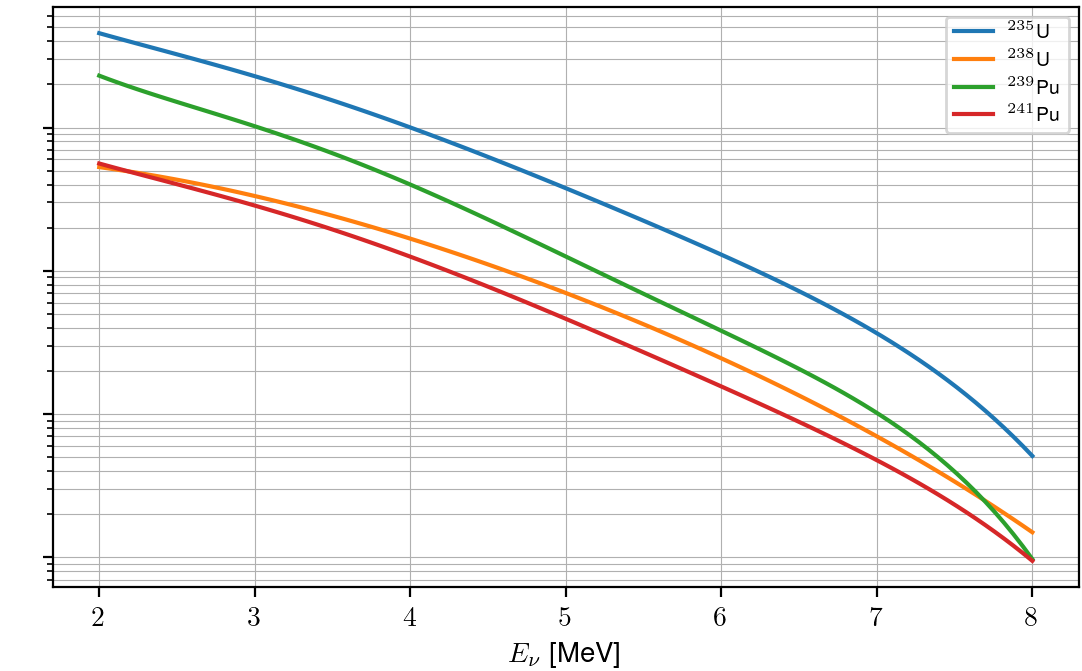
\includegraphics[width=0.8\textwidth]{figures/reactor_separate_crop.png}
    \caption{Isotope contributions to total antineutrino flux spectrum.}
    \label{fig:reator_sperate}
\end{figure}

\begin{figure}
    \centering
    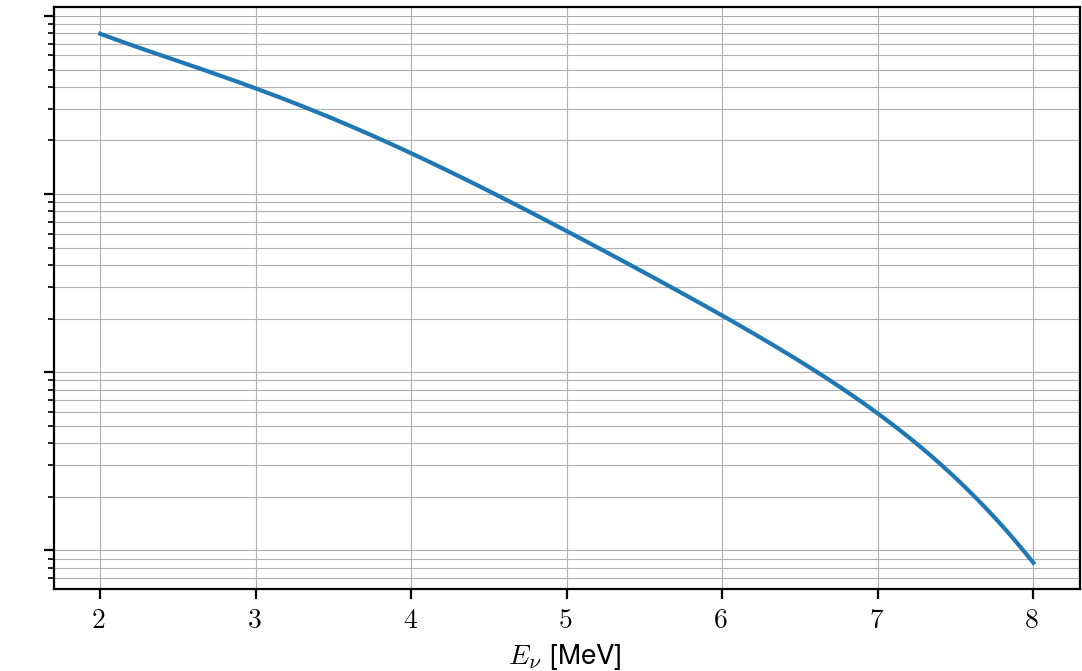
\includegraphics[width=0.8\textwidth]{figures/reactor_total_crop.png}
    \caption{Total antineutrino flux spectrum.}
    \label{fig:reator_total}
\end{figure}

\section{Expected Number of Events}
Ignoring reactor resolution and efficiency, the expected number of events of a detector of mass $M$ over an exposure time $t$ is given by
\begin{equation}
    N =  t\frac{M_{\text{Detector}}}{M}\int_{E_{R\text{ th}}}^{E_{R\text{ max}}}dE_R\int_{E_{\nu, \text{min}}(E_R)}^{E_{\nu,\text{max}}}dE_{\nu} \frac{d\Phi}{dE_\nu} (E_{\nu})\left( \frac{d\sigma}{dE_R}\right),
    \label{eq:N_events}
\end{equation}
where $E_{R\text{ th}}$ a threshold nuclear recoil energy, $E_{R\text{ max}}$ a kinematically determined maximum recoil energy, $E_{\nu,\text{max}}\sim9.5$ MeV the maximum incident neutrino energy given by the neutrino spectrum~\cite{SCHRECKENBACH1985325} and $E_{\nu, \text{min}}(E_R)\approx \sqrt{ME_R/2}$ the minimum incident neutrino energy required to produce a given $E_R$ recoil energy
\begin{equation}
    E_{\nu,\text{min}}(E_{R}) = \frac{E_{R}}{2}\left(1+\sqrt{1+\frac{2M}{E_{R}}}\right).
\end{equation}
